\subsubsection{Understanding NMT Weights}
\label{subsubsec:lstm}
\begin{figure*}[t]
\centering
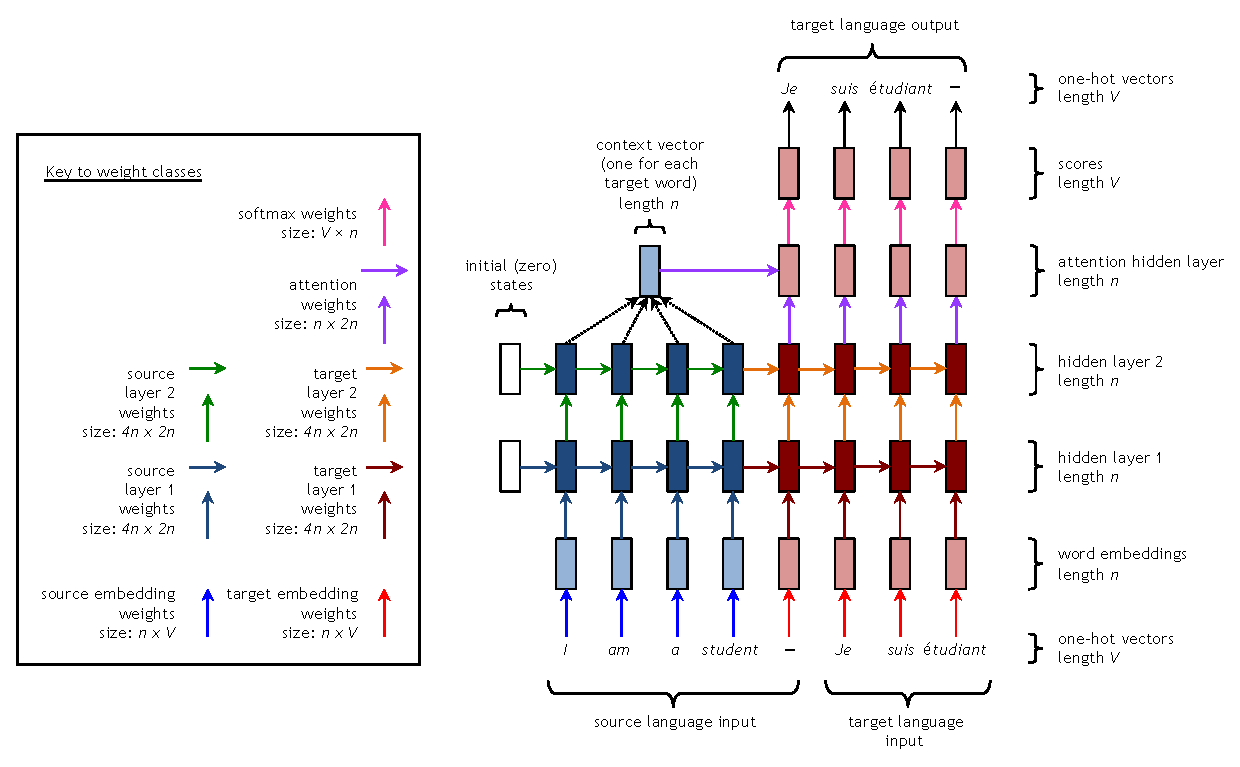
\includegraphics[width=\textwidth]{img/6-2_nmt_complex} %trim = 27mm 60mm 45mm 35mm, clip, 
\caption[Weights of NMT architecture]{NMT architecture. This example has two layers, but my system has four. The different weight classes are indicated by arrows of different color (the black arrows in the top right represent simply choosing the highest-scoring word, and thus require no parameters).
Best viewed in color.
}
\label{fig:nmt_complex}
\end{figure*}

In this work, I am focusing on the {\it deep multi-layer recurrent} architecture with {\it
LSTM} as the hidden unit type.
Figure~\ref{fig:nmt_complex} shows the system in detail,
highlighting the different types of parameters, or weights, in the model.
I will go through the architecture from bottom to top.
First, a vocabulary is chosen for each language, assuming that the top $V$ frequent
words are selected.
Thus, every word in the source or target vocabulary can be represented by a one-hot vector of length $V$.
The source input sentence and target input sentence, represented as a sequence
of one-hot vectors, are transformed into a sequence of word embeddings by the
\emph{embedding} weights. 
These embedding weights, which are learned during training, are different for the source words and the target words.
The word embeddings and all hidden layers are vectors of length $n$ (a chosen hyperparameter).

The word embeddings are then fed as input into the main network, which consists
of two multi-layer RNNs `stuck together' --- an encoder for the source
language and a decoder for the target language, each with their own
weights. 
The \emph{feed-forward} (vertical) weights connect
the hidden unit from the layer below to the upper RNN block, and the
\emph{recurrent} (horizontal) weights connect the hidden unit from the previous
time-step RNN block to the current time-step RNN block.
The hidden state at the top layer of the decoder is fed through an
\textit{attention} layer, which guides the translation by `paying attention'
to relevant parts of the source sentence.
Finally, for each target word, the top layer hidden unit is transformed by the
\emph{softmax} weights into a score vector of length $V$. The target word with the highest score is selected as the output translation.

{\it Weight Subgroups in LSTM} -- For the aforementioned RNN block, I choose to
use LSTM as the hidden unit type. To facilitate my later discussion 
on the different subgroups of weights
within LSTM, recall the details of the LSTM presented in Chapter 2 (2.35-2.37):
\begin{align}
\begin{pmatrix}
i\\
f\\
o\\
\hat{h}
\end{pmatrix}
&=
\begin{pmatrix}
\text{sigm}\\
\text{sigm}\\
\text{sigm}\\
\text{tanh}
\end{pmatrix}
T_{4n,2n}
\begin{pmatrix}
h_t^{l-1}\\
h_{t-1}^l
\end{pmatrix} \label{eqn:lstm_1} \\
c_t^l&=f \circ c_{t-1}^l + i \circ \hat{h} \label{eqn:lstm_2} \\
h_t^l &= o \circ \text{tanh}(c_t^l) \label{eqn:lstm_3}
\end{align}
Each LSTM block at time $t$ and layer $l$ computes as output a pair of
hidden and memory vectors ($h_t^l$, $c_t^l$) given the previous pair
($h_{t-1}^l$, $c_{t-1}^l$) and an input vector $h_t^{l-1}$ (either from the LSTM block below or
the embedding weights if $l\!=\!1$). All of these vectors
have length $n$.
The core of a LSTM block is the weight matrix $T_{4n,2n}$ of size $4n \times
2n$. This matrix can be decomposed into 8 subgroups that are responsible for the
interactions between $\{$input gate $i$, forget gate $f$, output gate $o$,
input signal $\hat{h}\} \times \{$feed-forward input $h_t^{l-1}$, recurrent
input $h_{t-1}^l\}$.

%\subsection{Evaluation metrics}
%I evaluate my models by two measures: BLEU score and perplexity. 
%BLEU compares the output target sentence with the human-translated target sentence, and is measured on a scale from 0 (worst) to 100 (best).
%Perplexity is the exponential of the average loss per word, measured on a scale from 1 (best) to infinity (worst). 
%%For each output target word, the model produces scores for each word in the vocabulary, which are converted to a probability distribution over the vocabulary. 
%The \emph{loss} is the negative log probability of the correct word --- that is, the lower the system's certainty in choosing the correct word, the higher the loss.
%
%Both evaluation metrics are valuable. 
%BLEU measures a system's performance on the end-goal of machine translation, translation quality, whereas perplexity is the quantity minimized during training.
%BLEU is a `hard' measure of performance, as it is calculated based on the sentences produced by the network, whereas perplexity is a `softer', more fine-grained measure that takes into account not just whether the correct target word was produced, but the probability of producing the correct target word.
%I use both BLEU and perplexity in this paper, as appropriate.

\subsubsection{Pruning Schemes}
\label{subsubsec:approach_schemes}
I follow the general magnitude-based approach of \cite{han2015learning}, which consists of pruning weights with smallest absolute value. However, I question the authors' pruning scheme with respect to the different weight classes, and experiment with three pruning schemes.
Suppose I wish to prune $x$\% of the total parameters in the model. 
How do I distribute the pruning over the different weight classes (illustrated in Figure~\ref{fig:nmt_complex}) of my model? 
I propose to examine three different pruning schemes:
\begin{enumerate}
\item \textit{Class-blind}: 
Take all parameters, sort them by magnitude and prune the $x$\% with smallest magnitude, regardless of weight class.
(So some classes are pruned proportionally more than others).
\item \textit{Class-uniform}: 
Within each class, sort the weights by magnitude and prune the $x$\% with smallest magnitude.
(So all classes have exactly $x$\% of their parameters pruned).
\item \textit{Class-distribution}: 
 For each class $c$, weights with magnitude less than $\lambda \sigma_c$ are
 pruned. Here, $\sigma_c$ is the standard deviation of that class and $\lambda$ is a universal parameter chosen such that in total, $x\%$ of all parameters are pruned.
This is used by \cite{han2015learning}.
\end{enumerate}
All these schemes have their seeming advantages.
Class-blind pruning is the simplest and adheres to the principle that pruning
weights (or equivalently, setting them to zero) is least damaging when
those weights are small, regardless of their locations in the architecture.
Class-uniform pruning and class-distribution pruning both seek to prune
proportionally within each weight class, either absolutely, or relative to the
standard deviation of that class.
I find that class-blind pruning outperforms both other schemes (see
Section~\ref{subsubsec:exp_schemes}).

\subsubsection{Retraining}
\label{subsubsec:approach_retraining}
In order to prune NMT models aggressively without performance loss, I retrain my pruned networks. 
That is, I continue to train the remaining weights, but maintain the sparse structure introduced by pruning.
In my implementation, pruned weights are represented by zeros in the weight matrices, 
and I use binary `mask' matrices, which represent the sparse structure of a network, 
to ignore updates to weights at pruned locations.
This implementation has the advantage of simplicity as it requires minimal changes to the training and deployment code, 
but I note that a more complex implementation utilizing sparse matrices and sparse matrix multiplication could potentially yield speed improvements.
However, such an implementation is beyond the scope of this work.

\begin{figure}
\centering
% !TEX root = acl2016.tex

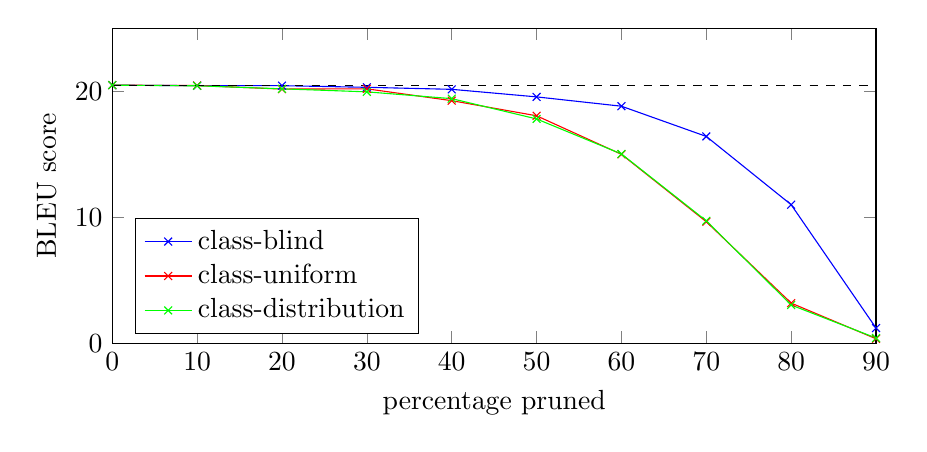
\begin{tikzpicture}

\begin{axis}[%
width=0.8\columnwidth,
height=4cm,
%at={(0\figurewidth,0\figureheight)},
scale only axis,
xmin=0,
xmax=90,
xtick={0, 10, 20, 30, 40, 50, 60, 70, 80, 90},
xlabel={percentage pruned},
%ymode=log,
ymin=0,
ymax=25,
yminorticks=true,
ylabel={BLEU score},
axis background/.style={fill=white},
legend pos = south west,
legend cell align=left
]
\addplot [color=blue,solid,mark=x,mark options={solid}]
  table[row sep=crcr]{%
  0	20.48\\
10	20.44\\
20	20.44\\
30	20.31\\
40	20.15\\
50	19.55\\
60	18.81\\
70	16.41\\
80	10.99\\
90	1.2\\
};
\addlegendentry{class-blind}

\addplot [color=red,solid,mark=x,mark options={solid}]
  table[row sep=crcr]{%
    0	20.48\\
10	20.45\\
20	20.17\\
30	20.19\\
40	19.25\\
50	18.05\\
60	14.99\\
70	9.64\\
80	3.18\\
90	0.35\\
};
\addlegendentry{class-uniform}

\addplot [color=green,solid,mark=x,mark options={solid}]
  table[row sep=crcr]{%
    0	20.48\\
10	20.43\\
20	20.19\\
30	19.95\\
40	19.41\\
50	17.8\\
60	15.02\\
70	9.71\\
80	3.03\\
90	0.41\\
};
\addlegendentry{class-distribution}

\addplot [color=black,dashed]
  table[row sep=crcr]{%
0	20.48\\
90	20.48\\
};
\end{axis}
\end{tikzpicture}%
\caption{Effects of different pruning schemes.}
\label{fig:pruning_methods}
\end{figure}

\begin{figure*}
\centering
% !TEX root = acl2016.tex


%\begin{tikzpicture}
%    \begin{axis}[
%width=0.8\textwidth,
%height=8cm,
%%at={(0\figurewidth,0\figureheight)},
%%scale only axis,
%        major y tick style = transparent,
%        xbar,
%        bar width=4pt,
%        xmajorgrids = true,
%        xlabel = {perplexity change},
%        symbolic y coords={source layer 1, source layer 2, source layer 3, source layer 4, target layer 1, target layer 2, target layer 3, target layer 4, attention, top layer, source embedding, target embedding},
%        ytick = data,
%        y=20pt,
%        scaled x ticks = false,
%     legend pos = south east,   
%    ]
%        \addplot[style={blue,fill=blue!50,mark=none}]
%            coordinates {(0.46659,source layer 1)  (0.362434,source layer 2)  (0.796254,source layer 3)  (0.794582,source layer 4)  (0.201001,target layer 1)  (0.222658,target layer 2)  (-0.291916,target layer 3)  (1.108432,target layer 4)  (0.4164,attention)  (7.803921,top layer)  (2.962925,source embedding)  (2.351362,target embedding)  };
%            
%        \addplot[style={red,fill=red!50,mark=none}]
%            coordinates {(0.471137,source layer 1)  (0.561763,source layer 2)  (1.829927,source layer 3)  (3.628541,source layer 4)  (0.422055,target layer 1)  (0.457759,target layer 2)  (0.473893,target layer 3)  (7.545939,target layer 4)  (6.362093,attention)  (16.277336,top layer)  (0.335614,source embedding)  (0.226382,target embedding)  };
%
%        \addplot[style={green,fill=green!50,mark=none}]
%            coordinates {(0.458798,source layer 1)  (0.543843,source layer 2)  (1.818222,source layer 3)  (3.93477,source layer 4)  (0.428267,target layer 1)  (0.46657,target layer 2)  (0.494273,target layer 3)  (8.308794,target layer 4)  (6.34294,attention)  (15.723167,top layer)  (0.311599,source embedding)  (0.253745,target embedding) };
%
%
%        \legend{delete smallest, uniform, standard deviation}
%    \end{axis}
%\end{tikzpicture}




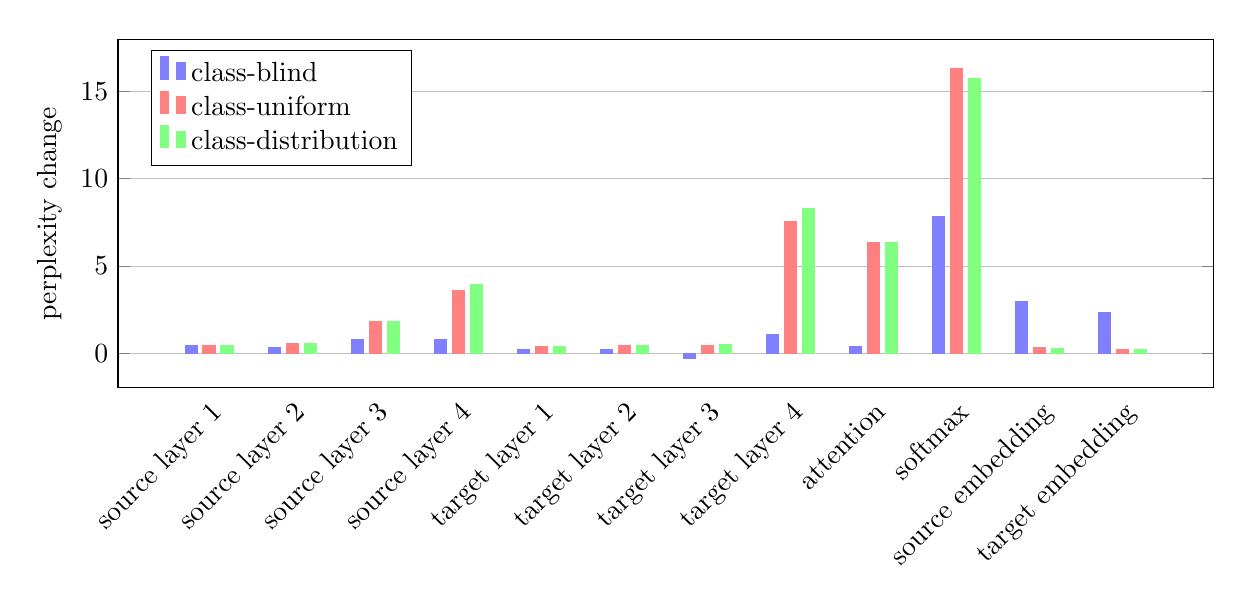
\begin{tikzpicture}
    \begin{axis}[
width=\textwidth,
height=6cm,
%at={(0\figurewidth,0\figureheight)},
%scale only axis,
        major x tick style = transparent,
        ybar,
        bar width=4.5pt,
        ymajorgrids = true,
        ylabel = {perplexity change},
        symbolic x coords={source layer 1, source layer 2, source layer 3, source layer 4, target layer 1, target layer 2, target layer 3, target layer 4, attention, softmax, source embedding, target embedding},
        x tick label style={rotate=45, anchor=north east, inner sep=0mm}, % inner sep controls how close the labels are to the plot
        xtick = data,
        x=30pt, % gap between groups of bars
        scaled y ticks = false,
     legend pos = north west,   
     legend cell align = left,
    ]
        \addplot[style={blue!50,fill=blue!50,mark=none}]
            coordinates {(source layer 1,0.46659)  (source layer 2,0.362434)  (source layer 3,0.796254)  (source layer 4,0.794582)  (target layer 1,0.201001)  (target layer 2,0.222658)  (target layer 3,-0.291916)  (target layer 4,1.108432)  (attention,0.4164)  (softmax,7.803921)  (source embedding,2.962925)  (target embedding,2.351362)};
            
        \addplot[style={red!50,fill=red!50,mark=none}]
            coordinates {(source layer 1,0.471137)  (source layer 2,0.561763)  (source layer 3,1.829927)  (source layer 4,3.628541)  (target layer 1,0.422055)  (target layer 2,0.457759)  (target layer 3,0.473893)  (target layer 4,7.545939)  (attention,6.362093)  (softmax,16.277336)  (source embedding,0.335614)  (target embedding,0.226382) };

        \addplot[style={green!50,fill=green!50,mark=none}]
            coordinates {(source layer 1,0.458798)  (source layer 2,0.543843)  (source layer 3,1.818222)  (source layer 4,3.93477)  (target layer 1,0.428267)  (target layer 2,0.46657)  (target layer 3,0.494273)  (target layer 4,8.308794)  (attention,6.34294)  (softmax,15.723167)  (source embedding,0.311599)  (target embedding,0.253745) 
 };
        \legend{class-blind, class-uniform, class-distribution}
    \end{axis}
\end{tikzpicture}
\caption[`Breakdown' of performance loss]{`Breakdown' of performance loss (i.e., perplexity increase) by weight class, when pruning 90\% of weights using each of the three pruning schemes. Each of the first eight classes have 8 million weights, attention has 2 million, and the last three have 50 million weights each.}
\label{fig:breakdown}
\end{figure*}


